%
% WORKS'13
%
\documentclass[final]{IEEEtran}
\hyphenation{op-tical net-works semi-conduc-tor}

\usepackage{makeidx}  % allows for indexgeneration
\usepackage{algorithm,algpseudocode}
\usepackage{graphicx}
\usepackage{float}
\usepackage{subcaption}
\captionsetup{compatibility=false}
\usepackage{wrapfig}
\usepackage{array}
\usepackage{cite}

\begin{document}

\title{Overhead Robustness of Scheduling Heuristics in Scientific Workflows}

\author{
  \IEEEauthorblockN{
    Weiwei Chen\IEEEauthorrefmark{1}, 
    Rafael Ferreira da Silva\IEEEauthorrefmark{3}, 
    Ewa Deelman\IEEEauthorrefmark{1},
    Rizos Sakellariou\IEEEauthorrefmark{4}\\
  }
  \IEEEauthorblockA{
     \IEEEauthorrefmark{1}University of Southern California, Information Sciences Institute, Marina Del Rey, CA, USA\\
     \{wchen,deelman\}@isi.edu \\
  }
  \IEEEauthorblockA{
    \IEEEauthorrefmark{3}University of Lyon, CNRS, INSERM, CREATIS, Villeurbanne, France\\
    rafael.silva@creatis.insa-lyon.fr \\
  }
  \IEEEauthorblockA{
    \IEEEauthorrefmark{4}University of Manchester, School of Computer Science, Manchester, U.K.\\
    rizos@cs.man.ac.uk
  }
}
\maketitle


\begin{abstract}
Workflow overheads play an important role in workflow performance particularly the scheduling performance. However, existing task scheduling strategies only provide a coarse-grained approach that relies on an over-simplified workflow model that ignores or underestimate the impact of overheads. In this work, we first identify the major overhead patterns in a general workflow management system. Next, we evaluate the performance of existing scheduling heuristics while varying overhead parameters (duration, etc.). Finally, we propose overhead robust heuristics that leverage overhead patterns even without a overhead duration prediction to improve the reliability of scheduling algorithms. A trace-based simulation of three popular scientific workflows shows scheduling heuristics that can release more jobs as soon as possible are more overhead robust because overheads may increase periodically. 



\end{abstract}

\begin{IEEEkeywords}
scientific workflow, scheduling, system overhead, log analysis
\end{IEEEkeywords}

\IEEEpeerreviewmaketitle


% Section
\section{Introduction}

Many computational scientists develop and use large-scale, loosely-coupled applications that are often structured as scientific workflows, which consist of many computational tasks with data dependencies between them. When executing these applications on a multi-machine distributed environment, such as the Grid or the Cloud, significant system overheads may exist~\cite{Chen, Prodan2008b, Dong2010, Yang03, WorkflowSim} and the problem of choosing robust schedules becomes more and more important. Traditionally, a carefully crafted schedule is based on deterministic or statistic estimates for the execution time of computational activities that compose a workflow. However, in such an environment, this approach may prove to be grossly inefficient~\cite{WorkflowSim}, as a result of various unpredictable overheads that may occur at runtime. 
%Particularly, it is challenging to provide a good estimate of overheads since it involves a lot of uncertainties. 
Thus, to mitigate the impact of uncertain overheads, it is necessary to choose a schedule that guarantees overhead robustness, that is, a schedule that is affected as little as possible by various overhead changes.  

There are several ways to achieve overhead robustness. A first approach is to integrate the overhead estimation into the job scheduling problem. A static or statistic estimation of communication cost or data transfer delay~\cite{Dong2010, Yang03} has been considered in the scheduling problem. Once we have the deterministic or statistic information of overheads, we can treat the system overhead as computational activities and the goal is to minimize the overall runtime including overhead duration. However, this approach only applies to the estimation of data transfer delay since the highly unpredictable variability and variety of other overheads make it a challenging work and not efficient in practice. Our prior work~\cite{Chen} has shown the variation of overheads may be comparable to the job runtime and thus makes it unrealistic in a real environment.  

A significant amount of work~\cite{Ahmad1998, Chetto1990, Dong2010, Yang03} in the literature has focused on proposing algorithms that are aware of the dynamic changes of runtime environments. Task rescheduling~\cite{Sakellariou2004, Zhang2009, Chen2010} is a typical approach that dynamically allocates tasks to an idle processor in order to take into account information that has been made available during the execution. Specifically, resource load~\cite{Dong2010} can be used to estimate the variance. However, rescheduling a task is costly as it implies some extra communication and synchronization costs. Relevant studies~\cite{Sakellariou2004} indicate that it is important to have a static schedule with good properties before the start of the execution. Therefore, even if a dynamic strategy is used, a good initial placement would reduce the possibility of making a bad decision. 

Another approach is to overestimate the execution time of individual jobs. Delay scheduling~\cite{Zaharia10} waits for a small amount of time, letting other MapReduce jobs launch tasks instead and this method can achieve a better tradeoff of locality and fairness. However, this method only applies to workload scheduling and particularly MapReduce jobs since the duration of them is short and thus it is not difficult to estimate the scheduling delay. Also, this results in a waste of resources as it induces a lot of idle time during the execution, if the overhead is shorter than the estimation. Second, overheads do not simply work as an attachment to the job runtime and it involves a lot more complicated patterns such as periodicity~\cite{Chen}. 

In this paper, we first present our work on evaluating the overhead robustness of scheduling heuristics and we indicate a list of heuristics that are overhead robust even without an estimate of the overhead duration. Second, since the estimate of overhead duration is difficult, we develop new heuristics that leverage the pattern information of workflow overheads, which represents a new approach to design overhead robust algorithms. To the best of our knowledge, so far, no study has systematically tried to evaluate the scheduling heuristics with respect to the overhead robustness.  

%To the best of our knowledge, this study is the first example of overhead robustness of scheduling heuristics and algorithms. 
The next Section gives an overview of the related work, Section~\ref{sec:model} presents our workflow and execution environment models, Section~\ref{sec:heuristics} details our heuristics and algorithms, Section~\ref{sec:experiments} reports experiments and results, and the paper closes with a discussion and conclusions.



\section{Related Work}

Some work in the literature has attempted to define and model robustness. In~\cite{Ali2004}, the authors propose a general method to define a metric for robustness. First, a performance metric is chosen. In our case, this performance metric is the overall runtime including overhead duration as we want the execution time of an application to be as stable as possible. Second, one has to identify the parameters that make the performance metric uncertain. In our case, it is the duration of the individual overheads. Third, one needs to find how a modification of these parameters changes the value of the performance metric. In our case, the answer is, as an increase of the overhead generally implies an increase of the overall runtime. 
%Lastly, one has to identify the smallest variation of a parameter that makes the performance metric exceed an acceptable bound. 
A schedule $A$ is said to be more robust than another schedule $B$ if the variation for $A$ is larger than that for $B$.
%However, estimating this variation is the most difficult part as it requires to analyze deeply the structure of the problem and its inputs.
Following this approach, Canon~\cite{Canon2008} analyzed the robustness of 20 static DAG scheduling heuristics using a metric for robustness the standard deviation of the makespan over a large number of measurement. Braun et al. \cite{Braun2001} evaluated 11 heuristics examined and for the cases studied there, the relatively simple Min-min heuristic performs well in comparison to the other techniques. In comparison, we focus on varying the parameters related to overhead instead of computational tasks. 

A plethora of studies on task scheduling~\cite{Chetto1990, Dong2010, Yang03, Blythe2005} have been developed in the distributed and parallel computing domains. Many of these schedulers have been extended to consider both the computational cost and communication cost. A static or statistic estimation of communication cost or data transfer delay~\cite{Dong2010, Yang03} has been considered in the scheduling problem. In contrast, we focus on the scheduling overheads that have been ignored or underestimated for long and we demonstrate how their unique timeline patterns influence the overhead robustness. 

Workflow patterns~\cite{Yu2005, Juve2013, Liu2008} are used to capture and abstract the common structure within a workflow and they give insights on designing new workflows and optimization methods.  
Yu~\cite{Yu2005} proposed a taxonomy that characterizes and classifies various approaches for building and executing workflows on Grids. They also provided a survey of several representative Grid workflow systems developed by various projects world-wide to demonstrate the comprehensiveness of the taxonomy. Juve~\cite{Juve2013} provided a characterization of workflow from 6 scientific applications and obtained task-level performance metrics (I/O, CPU and memory consumption). They also presented an execution profile for each workflow running at a typical scale and managed by the Pegasus workflow management system~\cite{Deelman2005}. Liu~\cite{Liu2008} proposed a novel pattern 
based time-series forecasting strategy which ulitilizes a 
periodical sampling plan to build representative 
duration series. Compared to them, we discover a common pattern of intervals existing in system overheads while executing scientific workflows. We also leverage this knowledge to evaluate the overhead robustness of existing heuristics and develop new heuristics. 

Overhead analysis \cite{Prodan2008b}\cite{Chen} is a topic of great interest in the grid community. Stratan \cite{Stratan} evaluates workflow engines including DAGMan/Condor and Karajan/Globus in a real-world grid environment. Sonmez \cite{Sonmez} investigated the prediction of the queue delay in grids and assessed the performance and benefit of predicting queue delays based on traces gathered from various resource and production grid environments. Prodan \cite{Prodan2008b} offers a grid workflow overhead classification and a systematic measurement of overheads. Our prior work \cite{Chen} further investigated the major overheads and their relationship with different optimization techniques. In this paper, we leverage these knowledge to enhance the existing scheduling heuristics and provide insights on designing new algorithms. 

%Braun paper
%Opportunistic Load Balancing, Minimum Execution Time, Minimum Completion Time, Min-min, Max-min, Duplex, Genetic Algorithm, Simulated Annealing, Genetic Simulated Annealing, Tabu, and A*

%The 11 static mapping heuristics were evaluated using simulated execution times for an HC environment. Because these are static heuristics, it is assumed that an accurate estimate of the expected execution time for each task on each machine is known prior to execution and contained within a  ETC (expected time to compute) matrix. The assumption that these estimated expected execution times are known is commonly made when studying mapping heuristics for HC systems (e.g., [19, 26, 40]). (Approaches for doing this estimation based on task profiling and analytical benchmarking are discussed in [27, 30, 37].)

%Data dependencies between workflow tasks play an important role when clustering tasks within a level. A data dependency means that there is a data transfer between two tasks (output data for one and input data for the other). Grouping tasks without considering these dependencies may lead to data locality problems where output data produced by parent tasks are poorly distributed. Thus, data transfer times and failures probability increase.Therefore, we claim that data dependencies of subsequent tasks should be considered.




%\textbf{Workflow Management Systems} (WMS) such as Askalon \cite{Fahringer}, Taverna \cite{Oinn}, and Pegasus \cite{Deelman} are designed to run scientific workflows on distributed environments. DAGs (Directed Acyclic Graph) and other task graph representations are widely used as the programming model for many parallel applications because it is effective in expressing and optimizing irregular computations. 
%Moreover, algorithms expressed as DAGs have the potential to alleviate the user from focusing on the architectural issues, while allowing the engine to extract the best performance from the underlying architecture. 




%Section
\section{Model and Design}

\label{sec:model}

\begin{figure}[htb]
	\centering
	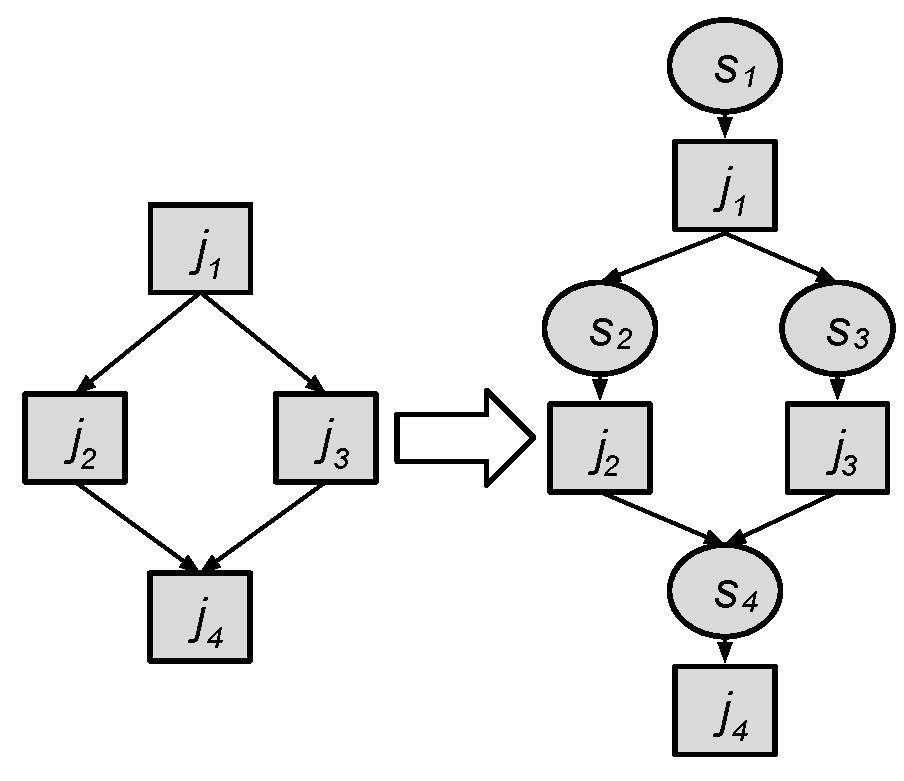
\includegraphics[width=0.7\linewidth]{figure/odag.pdf}
	\captionof{figure}{Extending DAG to o-DAG.}
	\label{fig:odag}
	\vspace{-10pt}
\end{figure}
A workflow is modeled as a Directed Acyclic Graph (DAG) as shown in \ref{fig:odag}. Each node in the DAG often represents a workflow job ($j$), and the edges represent dependencies between the jobs that constrain the order in which the jobs are executed. Dependencies typically represent data-flow dependencies in the application, where the output files produced by one job are used as inputs of another job. Each job is a single execution unit and it may contains one or multiple tasks, which is a program and a set of parameters that need to be executed. Fig.~\ref{fig:odag} (left) shows an illustration of a DAG composed by four jobs. This model fits several workflow management systems such as Pegasus~\cite{Deelman2005}, Askalon~\cite{Fahringer2005}, and Taverna~\cite{Oinn:2006:TLC:1148437.1148448}.


Fig.~\ref{fig:system} shows a typical workflow execution environment. The submit host prepares a workflow for execution (clustering, mapping, etc.), and worker nodes, at an execution site, execute jobs individually. The main components are introduced below:

\begin{figure}[htb]
\centering
  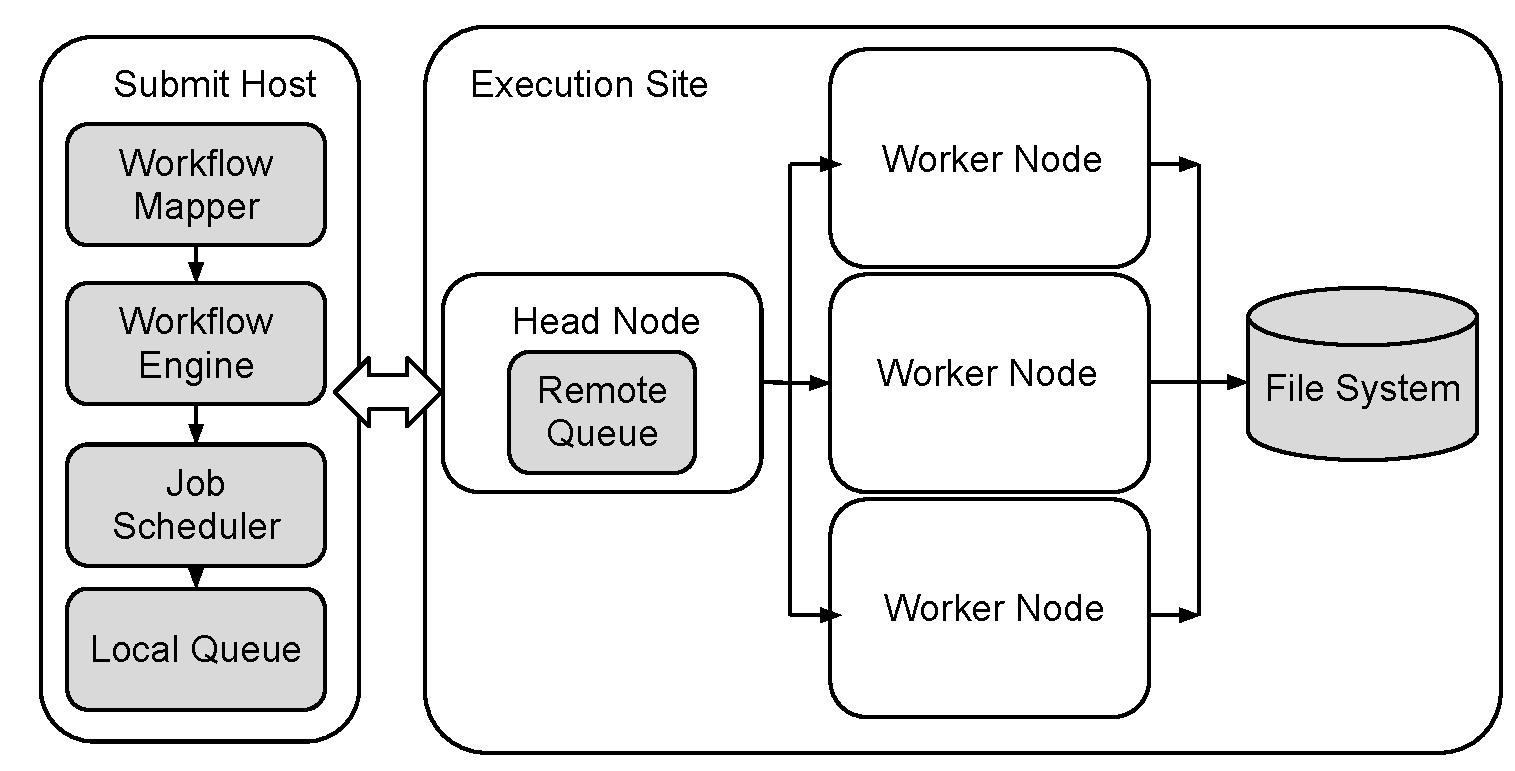
\includegraphics[width=0.95\linewidth]{figure/execution.pdf}
  \caption{A workflow system model.}
  \label{fig:system}
  \vspace{-10pt}
\end{figure}

\paragraph{Workflow Mapper} generates an executable workflow based on an abstract workflow provided by the user or workflow composition system. It also restructures the workflow to optimize performance and adds jobs for data management and provenance information generation. 

\paragraph{Workflow Engine} executes jobs defined by the workflow in order of their dependencies. Only jobs that have all their parent jobs completed are submitted to the Job Scheduler. Workflow Engine relies on the resources (compute, storage, and network) defined in the executable workflow to perform the necessary actions. The time period when a job is free (all of its parents have completed successfully) to when it is submitted to the job scheduler is denoted the workflow engine delay. The workflow engine delay is usually configured by users to assure that the entire workflow scheduling and execution system is not overloaded. 

\begin{figure}[htb]
\centering
 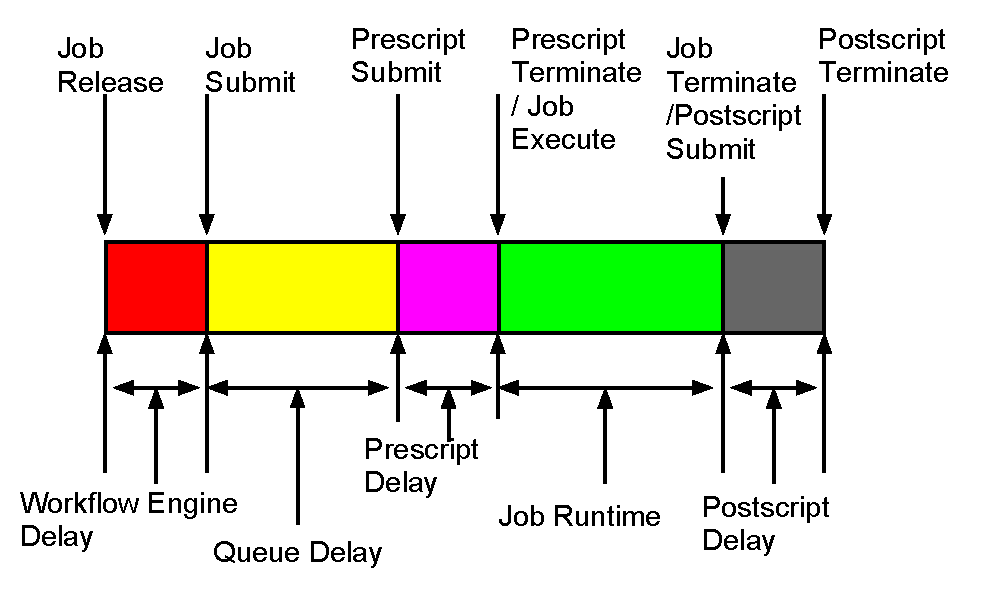
\includegraphics[width=1\linewidth]{figure/timeline.pdf}
  \captionof{figure}{Overhead Classification}
  \label{fig:overhead}
  \vspace{-10pt}
\end{figure}

\paragraph{Job Scheduler and Local Queue} manage individual workflow jobs and supervise their execution on local and remote resources. The time period when a job is submitted to the job scheduler to when the job starts its execution in a worker node is denoted the queue delay. It reflects both the efficiency of the job scheduler and the resource availability. 


The execution of a job is comprised of a series of events as shown in Figure~\ref{fig:overhead} and they are defined as:
\begin{enumerate}
\item Job Release is defined as the time when the workflow engine identifies that a job is ready to be submitted (when its parents have successfully completed). 
\item Job Submit is defined as the time when the workflow engine submits a job to the local queue. 
\item Job Execute is defined as the time when the workflow engine sees a job is being executed. 
\item Task Execute is defined as the time when the job wrapper sees a task is being executed. 
\item Pre/Postscript Start is defined as the time when the workflow engine starts to execute a pre/postscript. 
\item Pre/Postscript Terminate is defined as the time when the pre/postscript returns a status code (success or failure). 
\end{enumerate}

Figure~\ref{fig:overhead} shows a typical timeline of overheads and runtime in a compute job. We do not specify the data transfer delay in this timeline because data transfer is handled by data transfer jobs (stage-in and stage-out jobs). 

As shown in our prior work \cite{Chen}, we have classified workflow overheads into three categories as follows. 
\begin{enumerate}

\item{Workflow Engine Delay} measures the time between when the last parent job of a job completes and the time when the job gets submitted to the local queue. The completion time of the last parent job means this job is released to the ready queue and is waiting for resources to be assigned to it. The workflow engine delay reflects the efficiency of a workflow engine (i.e., DAGMan~\cite{DAGMan}). 

\item{Queue Delay} is defined as the time between the submission of a job by the workflow engine to the local queue and the time the local scheduler sees the job running. This overhead reflects the efficiency of the local workflow scheduler (e.g. Condor \cite{Frey2002}) to execute a job and the availability of resources for the execution of this job. 

\item{Pre/Postscript Delay } is the time taken to execute a lightweight script under some execution systems before/after the execution of a job. For example, prescripts prepare working environment before the execution of a job starts and postscripts examine the status code of a job after the computational part of this job is done.


\end{enumerate}

The overhead aware DAG model (o-DAG) we use in this work is an extension of the traditional DAG model. System overheads play an important role in workflow execution and constitute a major part of the overall runtime when jobs are poorly mapped to resources. Fig.~\ref{fig:odag} shows how we augment a DAG to be an o-DAG with the capability to represent system overheads ($s$) such as workflow engine delay and queue delay. 


In summary, an o-DAG representation allows the specification of high level system overhead details, which is more suitable for the study of overhead aware scheduling. 


\subsection{Overhead Patterns}

In this section, we introduce the common overhead patterns in workflow execution. 
In scientific workflow systems, time related functionalities such as workflow scheduling normally requires effective forecasting of activity patterns. In this work, we mainly focus on the overhead pattern that refers to a representative time series of overhead activities that occurs repeatedly and regularly in workflow execution. An overhead pattern is composed of ordered overhead activities obtained from scientific workflow system logs or other forms of historical data. 
Pattern discovery~\cite{Liu2008} usually starts from a periodical sampling plan to build representative duration series (Job Release, etc. ) and then conducts time-series segmentation to discover the pattern sets and predicts the activity duration intervals with pattern matching results. 


The motivation for pattern based analysis comes from the observation that for those duration-series segments where the number of concurrent activity instances is similar, these activity durations reveal comparable statistical features. Due to the dynamic nature of underlying resources, pattern based forecasting of overheads can improve the effectiveness of scheduling heuristics. 

\begin{figure}[htb]
\centering
 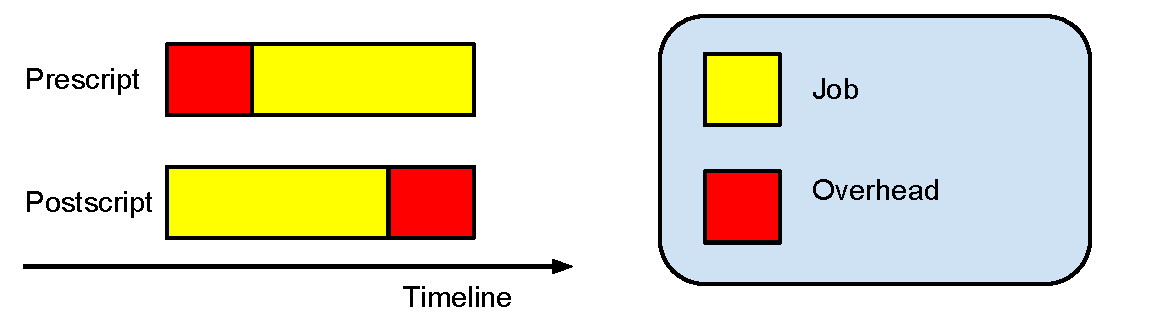
\includegraphics[width=1\linewidth]{figure/adherence.pdf}
  \captionof{figure}{Adherence Pattern}
  \label{fig:adhere}
  \vspace{-10pt}
\end{figure}

Most of the work~\cite{Dong2010, Yang03} view the overhead duration as an attachment to runtime in workflow timeline. For example, the Pre/Post-script Delay is usually constant, which we call it Adherence Pattern as shown in Fig.~\ref{fig:adhere}. Scheduling algorithms can just add the delay to the job runtime without significant change to the algorithms. For this pattern, we have shown in our prior work~\cite{Chen} that it does not have much influence on the overhead robustness. 
However, we observe that the Workflow Engine Delay and the Queue Delay increases periodically and steadily. For example, Fig.~\ref{fig:trace} shows the Gantt chart of part of a real trace\footnote{Details: http://www.isi.edu/\string~wchen/fgrid/run}. 
The Workflow Engine Delay (red) of the first 16 jobs is 5 seconds and then it increases to 10 seconds. 
%It is difficult to explain queue delay
We call this common overhead pattern the Incremental and Periodical Pattern (IPP). We observe the Queue Delay also increases periodically but the period is interrupted by the resource availability and thus it has a more complicated IPP. In the rest of this paper, we focus on the IPP of the Workflow Engine Delay and we will cover the Queue Delay in our future work. 
The reason why IPP prevalently exists is that many workflow management components are queue based systems. They repeatedly check their queues to find whether there are idle jobs, if yes they will process and submit these jobs, otherwise it will wait for a interval and continue. In Fig.~\ref{fig:ipp} we abstract the IPP from the trace, which shows a repeatedly increase by a interval. We define throughput of a workflow management component as the maximum number of allowed jobs in queue. For example, the interval and the throughput of the Workflow Engine in Fig.~\ref{fig:trace} are around 5 seconds and 16 respectively. 


\begin{figure}[htb]
\centering
 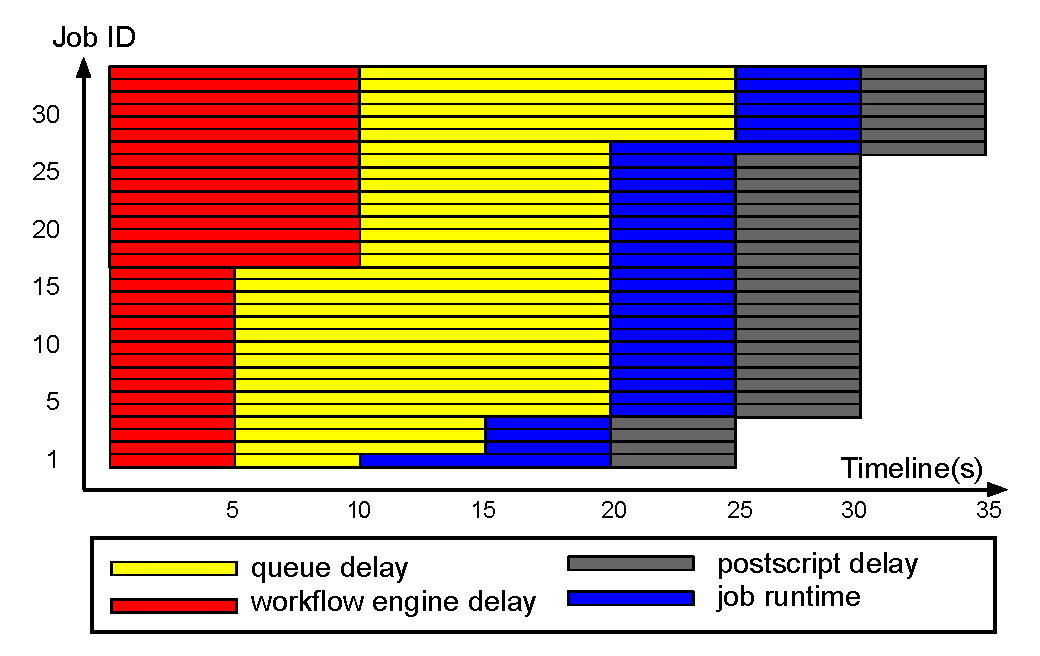
\includegraphics[width=1\linewidth]{figure/trace.pdf}
  \captionof{figure}{Workflow Execution Gantt Chart of a Real Trace}
  \label{fig:trace}
  \vspace{-10pt}
\end{figure}



%Some representative time series, including marketing time series, temperature time series and quality control time series, are effectively applied in various scientific and business domains [6][7]. Similarly, 

%Current forecasting strategies for computation tasks mainly reside on the prediction of CPU load [1][15], however, this is quite different from the prediction of scientific workflow activity durations.Activity durations cover the time intervals from the initial submission to the final completion of each workflow activity [3]. Hence, besides the exact execution time on scheduled resources, they also consist of extra time, i.e. scientific workflow overheads. According to [11], there exist four main categories of scientific workflow overheads, i.e. middleware overhead, data transfer overhead, loss of parallelism overhead and activity related overhead. Evidently, scientific workflow activity durations involve much more affecting factors than that of conventional computation tasks which are dominated by high performance computing resources.scientific workflow activity durations denote discrete long-term intervals since activity instances only occur occasionally and take several minutes or more than a couple of hours to complete.

%The motivation for pattern based time-series forecasting comes from the observation that for those duration-series segments where the number of concurrent activity instances is similar, these activity durations reveal comparable statistical features. 

These overhead patterns reappear frequently during a duration series and they represent unique behavior of the workflow management components. After we define and discover these typical patterns, the intervals and throughputs of these patterns can be estimated and statistically captured from historical traces. 



%Furthermore, if these overhead patterns reappear frequently during a duration series, they can be deemed as potential patterns which represent unique behavior of the duration-series under certain circumstances. Therefore, if we are able to define and discover these typical patterns, the intervals of future durations can be estimated with the statistical features of the closest patterns by matching the latest duration sequences. 





\begin{figure}[htb]
\centering
 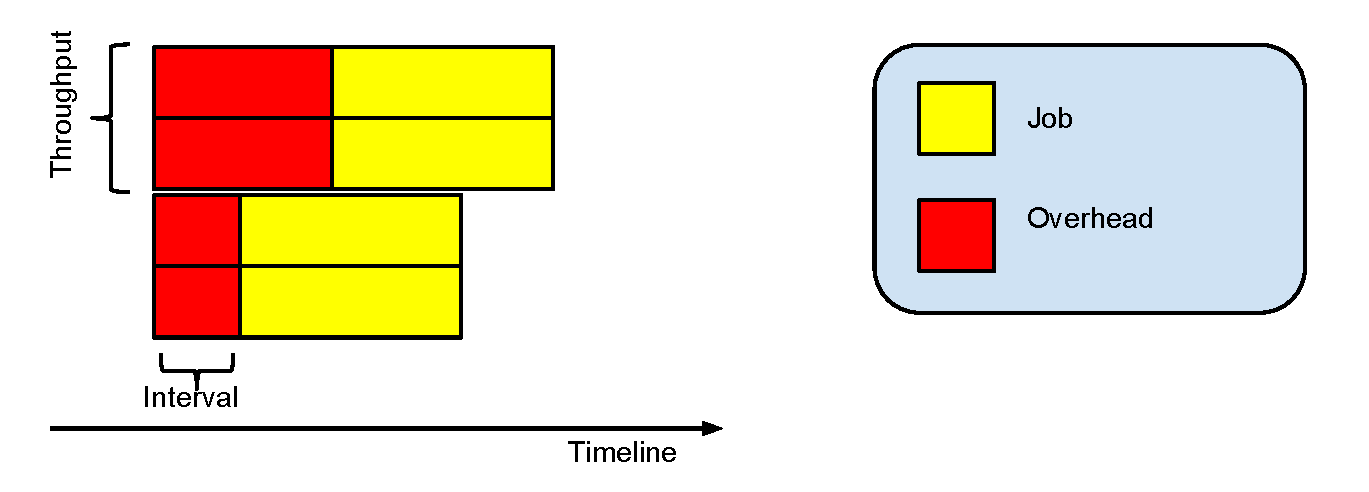
\includegraphics[width=1\linewidth]{figure/incremental.pdf}
  \captionof{figure}{Incremental and Periodical Pattern}
  \label{fig:ipp}
  \vspace{-10pt}
\end{figure}

%It is not workflow engine delay it is workflow engine interval
\section{Overhead Robust Heuristics}
\label{sec:heuristics}
In this section, we introduce the overhead robustness of four pairs of scheduling heuristics. Heuristics are widely used in workflow scheduling since the scheduling problem is a NP-hard problem and the time complicity of a global optimization of the overall runtime is not affordable. Usually, heuristics utilize unique features of workflows or resources to guide the mapping of jobs to resources. For example, both of the MINMIN~\cite{Blythe2005} algorithm and the MAXMIN~\cite{Braun2001} algorithm utilize the runtime of a job as the feature. However, they conduct the mapping in an opposite way, that is, MINMIN chooses the job with the shortest runtime while MAXMIN chooses the job with the longest runtime. Intuitively speaking, there must be either of them (we call it overhead robust) that performs better than the other one (we call it overhead unrobust) since they operates oppositely. Inspired by these coupling heuristics, we use a relative overhead robustness approach to evaluate these scheduling heuristics. For a pair of heuristics that use the same feature, we define the relative overhead robustness as the performance gain of the overhead robust heuristic against the other one. The more performance gain we have, the more significant this feature has on the overhead robustness. Also, it is not fair to compare scheduling heuristics that use different features because they may have vastly different performance even without overheads. Furthermore, in practice, we can use scheduling heuristics with different features at the same time but not those with the same features. 
Below we introduce the four pairs of scheduling heuristics including one that we propose. 

%OLB: Opportunistic Load Balancing (OLB) assigns each task, in arbitrary order, to the next machine that is expected to be available, regardless of the task's expected execution time on that machine [3, 17, 18]. The intuition behind OLB is to keep all machines as busy as possible. One advantage of OLB is its simplicity, but because OLB does not consider expected task execution times, the mappings it finds can result in very poor makespans.
%MET: In contrast to OLB, Minimum Execution Time ( MET ) assigns each task, in arbitrary order, to the machine with the best expected execution time for that task, regardless of that machine's availability [3, 17]. The motivation behind MET is to give each task to its best machine. This can cause a severe load imbalance across machines. In general, this heuristic is obviously not applicable to HC environments characterized by consistent ETC matrices.
%MCT: Minimum Completion Time (MCT) assigns each task, in arbitrary order, to the machine with the minimum expected completion time for that task [3]. This causes some tasks to be assigned to machines that do not have the minimum execution time for them. The intuition behind MCT is to combine the benefits of OLB and MET, while avoiding the circumstances in which OLB and MET perform poorly.

\emph{MINMIN} and \emph{MAXMIN}: The MINMIN heuristic begins with a set of all unmapped jobs. Then, the set of minimum completion times for each job, M namely, is found. Next, the job with the overall minimum completion time from M is selected and assigned to the corresponding resource (hence the name MINMIN). Last, the newly mapped job is removed from the unmapped jobs, and the process repeats until all jobs are mapped. 
%Minin maps the tasks in the order that changes the machine availability status by the least amount that any assignment could. Let ti be the first task mapped by Minin onto an empty system. The machine that finishes ti the earliest, say mj , is also the machine that executes ti the fastest. For every task that MINMIN maps after ti, the Minin heuristic changes the availability status of mj by the least possible amount for every assignment. Therefore, the percentage of tasks assigned to their first choice (on the basis of execution time) is likely to be higher for Minmin than for Maxin (defined next). The expectation is that a smaller makespan can be obtained if more tasks are assigned to the machines that complete them the earliest and also execute them the fastest.
The MAXMIN heuristic is very similar to MINMIN. The MAXMIN heuristic also begins with the set of all unmapped jobs. Then, the set of minimum completion times, M, is found. Next, the job with the overall maximum completion time from M is selected and assigned to the corresponding resource (hence the name MAXMIN). Last, the newly mapped job is removed from the unmapped jobs, and the process repeats until all jobs are mapped. 
Intuitively speaking, we believe MAXMIN has better overhead robustness than MINMIN. As shown in Fig.~\ref{fig:longest}, assuming we have two jobs and the interval of the overhead is 1. MAXMIN releases a job with longer runtime first, which can overlap with the increment of the overheads when MAXMIN releases the other job. However, the performance gain depends on the values of overhead interval, job runtime, overhead duration and the resource availability. 

\begin{figure}[htb]
\centering
 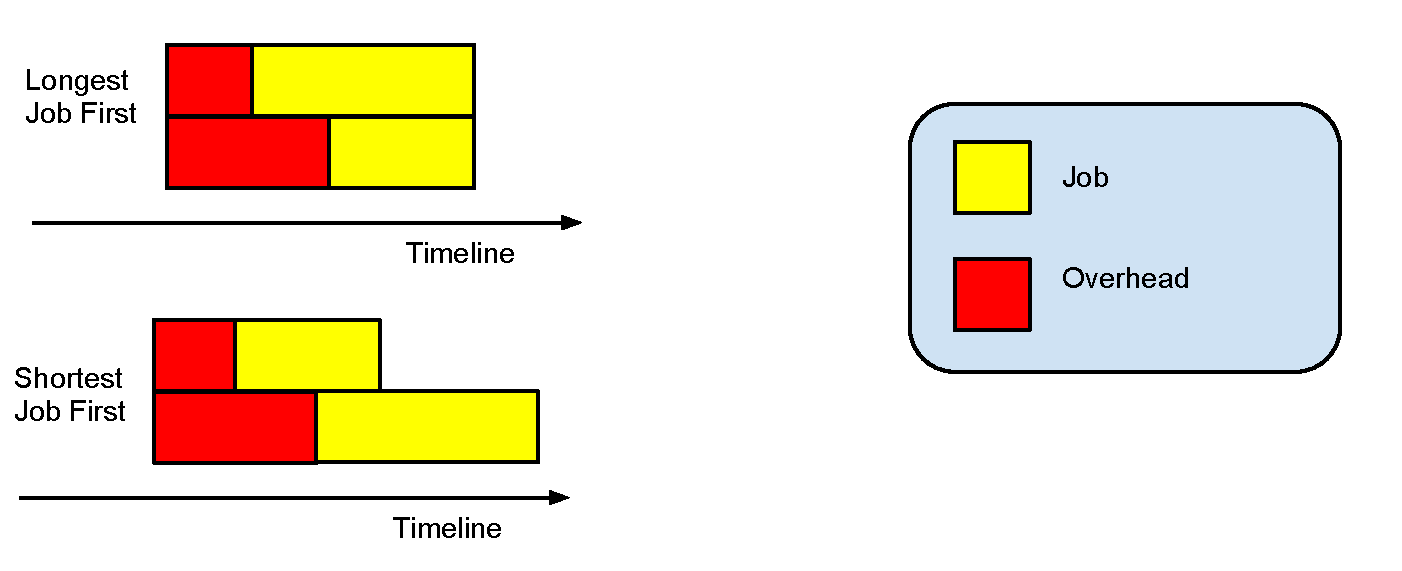
\includegraphics[width=1.0\linewidth]{figure/longest.pdf}
  \captionof{figure}{MAXMIN vs. MINMIN}
  \label{fig:longest}
  \vspace{-10pt}
\end{figure}
\emph{Breadth First} and \emph{Depth First}: Namely, the Breadth First (BFS) algorithm iterates the jobs at the same workflow level (or depth within a workflow directed acyclic graph) first while the Depth First (DFS) algorithm iterates the jobs at the deepest workflow level first. Intuitively speaking, we believe BFS performs better than DFS in terms of overhead robustness since BFS releases more jobs at the same workflow level for most scientific workflows as shown in Fig.~\ref{fig:shape}. Therefore, with enough jobs in queue, BFS can fully utilize the resources without wasting this overhead interval.  

\emph{Fertile First} and \emph{Unfertile First}: The Fertile First (FFS) algorithm sorts all the unmapped jobs based on the number of children jobs that they have and assigns the jobs with most children jobs first. The Unfertile First (UFFS) algorithm works in the opposite way and assigns the jobs with lest children jobs first. Similar to the case of BFS and DFS, we believe FFS should perform better than UFFS since FFS releases more jobs at the next level compared to UFFS and thus FFS can fully utilize the available resources. 

\begin{figure}[htb]
\centering
 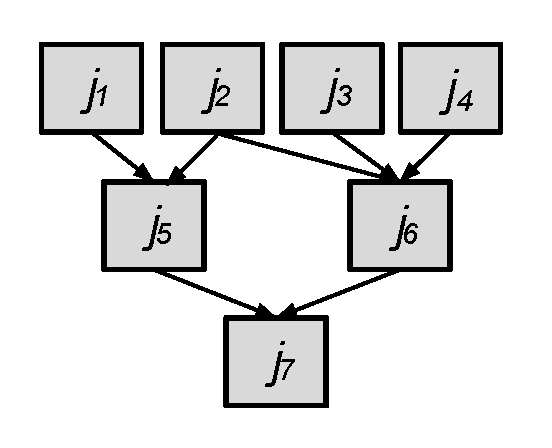
\includegraphics[width=0.6\linewidth]{figure/impact_factor.pdf}
  \captionof{figure}{Impact Factor}
  \label{fig:impact}
  \vspace{-10pt}
\end{figure}

\emph{Important First} and \emph{Unimportant First}: Here we propose a pair of Impact Factor based scheduling heuristics. The Important First (IFS) algorithm sorts all the unmapped jobs based on their \emph{Impact Factor} (IF) and assigns the jobs with the largest IF first while the Unimportant First (UIFS) algorithm assigns the jobs with the smallest IF first. 
The \textbf{Impact Factor} ($IF$) of a job $j_u$ is defined as follows:

\begin{equation}
	IF(j_u)=\sum_{j_v\in Child(j_u)}^{}\frac{IF(j_v)}{L(j_v)}
\end{equation}
where $Child(j_u)$ denotes the set of child jobs of $j_u$, and $L(j_v)$ the number of parent jobs of $j_v$. For simplicity, we assume the $IF$ of a workflow exit job (e.g. $j_7$ in Fig.~\ref{fig:impact}) as 1.0. For instance, consider the workflow in Fig.~\ref{fig:impact}. $IF$ for $j_1$, $j_2$, $j_3$, and $j_4$ are computed as follows:

\begin{eqnarray}
	\displaystyle  
	&IF(j_7 )=1.0, IF(j_6 )=IF(j_5 )=IF(j_7 )/2=0.5\nonumber  \\
	&IF(j_1 )=IF(j_5)/2=0.25\nonumber \\
	&IF(j_2 )=IF(j_5 )/2+IF(j_6)/3=0.42\nonumber \\
	&IF(j_3 )=IF(j_4 )=IF(j_6 )/3=0.17\nonumber 
\end{eqnarray}
Thus, IFS algorithm should schedule $j_2$ first while UIFS algorithm should schedule $j_3$ or $j_4$ first. The intuition of Impact Factor is that we aim to measure the relative importance of a job to the entire graph. Intuitively speaking, tasks with larger impact factors should have more impacts on the remaining jobs compared to tasks with smaller impact factors. For example, a bottleneck usually has a larger IF since it controls the release of more jobs. 
Similar to the case of FFS and UFFS, we believe IFS has a better overhead robustness than UIFS since IFS releases more jobs at the next few levels compared to UFFS. 


%The idea of these overhead aware heuristics is we would like to improve the overhead robustness even when we are not able to precisely predict the duration of overheads. Instead, workflow overheads have common patterns, which can determine the relative performance of different heuristics. 
Table~\ref{tab:heuristics} summaries the heuristics and their potential overhead robustness. 
\begin{table}[H]
\caption{Scheduling Heuristics}
\begin{center}
  \begin{tabular}{ l|l|l}
    \hline
Heuristics & Overhead Robust & Overhead Unrobust \\ \hline
    Experiment 1 & MAXMIN & MINMIN \\ \hline
   Experiment 2 & BFS & DFS \\ \hline
 Experiment 3 & FFS & UFFS \\ \hline
Experiment 4 & IFS & UIFS\\
    \hline
  \end{tabular}
\label{tab:heuristics}
\end{center}
\end{table}

% Section
\section{Experiment and Evaluation}
\label{sec:experiments}

The experiments presented hereafter evaluate the performance of the four pairs of heuristics mentioned ahead, which are widely used by workflow management systems. 

\subsection{Experiment Conditions}


\begin{figure}[htb]
	\centering
	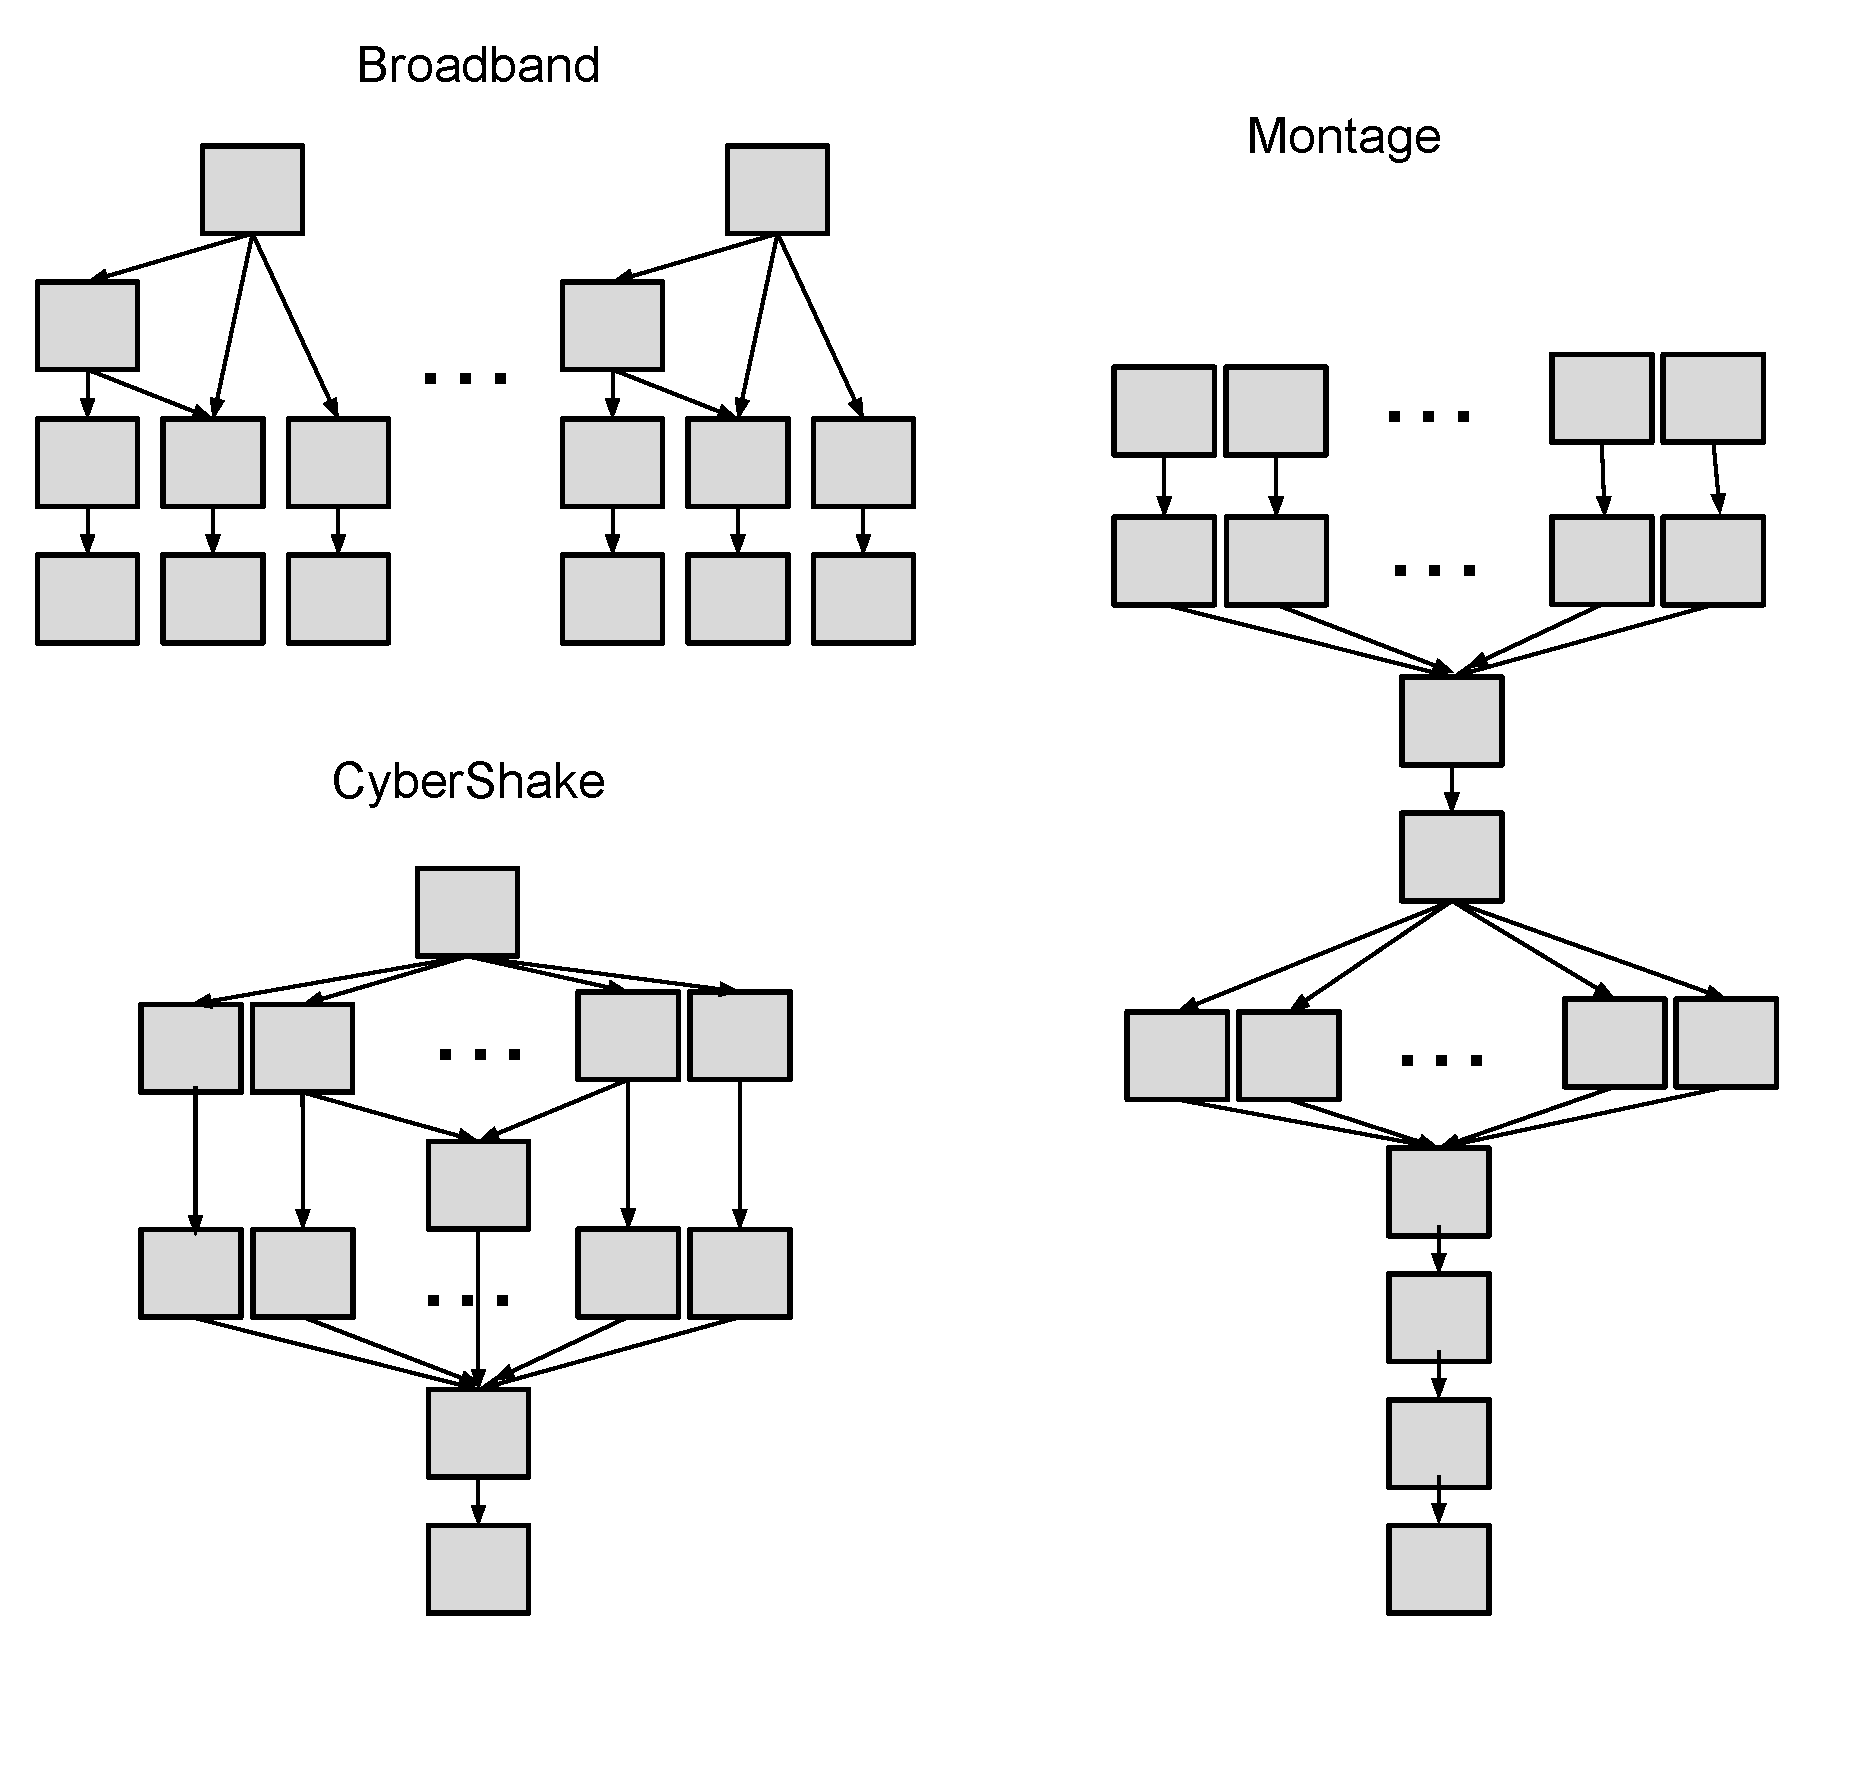
\includegraphics[width=1.0\linewidth]{figure/shape.pdf} 
	\caption{A simplified visualization of the Broadband workflow, the Montage workflow and the CyberShake workflow.}
	\label{fig:shape}
	\vspace{-10pt}
\end{figure}

We extended the WorkflowSim~\cite{WorkflowSim} simulator with the overhead model to simulate a distributed environment where we could evaluate the overhead robustness of scheduling algorithms when varying the average overheads and throughput. As an initial attempt, we focus on the workflow engine delay ($d$) in this paper. The simulated computing platform is composed by 20 single core virtual machines (worker nodes), which is the quota per user of some typical distributed environments such as Amazon EC2~\cite{AmazonAWS} and FutureGrid~\cite{FutureGrid}. Each machine has 512MB of memory and the capacity to process 1,000 million instructions per second. 
%Task scheduling is data-aware, i.e. tasks are scheduled to resources which have the most input data available.
%WorkflowSim is a feature-rich toolkit to simulate workflow planning and execution. It provides runtime randomization and multiple task clustering methods that we need. 



Three workflows are used in the experiments: 
Broadband~\cite{Broadband} is an application that enables researchers to combine long-period deterministic seismograms with high-frequency stochastic seismograms. 
Montage~\cite{Sakellariou2010} is an astronomy application used to construct large image mosaics of the sky. CyberShake~\cite{Callaghan2008} is a seismology application that calculates Probabilistic Seismic Hazard curves for geographic sites in the Southern California region. All workflows are generated and varied using the WorkflowGenerator\footnote[1]{https://confluence.pegasus.isi.edu/display/pegasus/WorkflowGenerator}. Each workflow instance is composed by around 100 tasks and its workflow structure is presented in Fig.~\ref{fig:shape}. Runtime (average and task runtime distribution) and overhead (workflow engine delay and queue delay) information were collected from real traces production environments~\cite{Chen, Juve2013}, then used as input parameters for the simulations.

%We first collected runtime information  (i.e., average and distribution of task runtime) and overhead information (including workflow engine delay, queue delay and network bandwidth) from the real traces that were run on real environments before. 
%Part of runtime distribution and overhead information were shown in \cite{Juve2013} and \cite{Chen} respectively. 
%Then we input these parameters into WorkflowSim and run these workflows repeatedly until the variance is less than 5\% of the average workflow runtime. 



Four sets of experiments are conducted. Experiment 1 evaluates the relative robustness of MAXMIN and MINMIN by comparing the performance gain of the overhead robust heuristic (MAXMIN in this experiment) over the overhead unrobust heuristic (MINMIN), while varying the average interval of workflow engine ($d$) and throughput of workflow engine ($t$). Table~\ref{tab:heuristics} shows the heuristics compared in these experiments. Simulation results present a confidence level of 95\%. Thus, for values of \emph{Performance Gain} $> 0$, the overhead robust heuristics perform better than the respective overhead unrobust heuristics. Otherwise, the overhead robust heuristics perform poorer.
%We randomly select 20\% from LIGO workflow tasks and increase their task runtime by a factor of \emph{Ratio} to simulate the system variation in a production environment.




In these experiment sets, we vary the average throughput of workflow engine from 1 to 20 and we show the results of $t=1, 5, 15, 20$. The original throughput of workflow engine in these traces is 5 and a throughput that is larger than 20 does not influence the performance much since we have only 20 worker nodes in our experiments. We also vary the average interval of workflow engine from 0 to 100 seconds, which represents a typical range of workflow engine delay as shown in~\cite{Chen} and this range is able to show the difference of overhead robustness in these heuristics. 

\subsection{Results and Discussion}

\begin{figure}[!htb]
\centering
 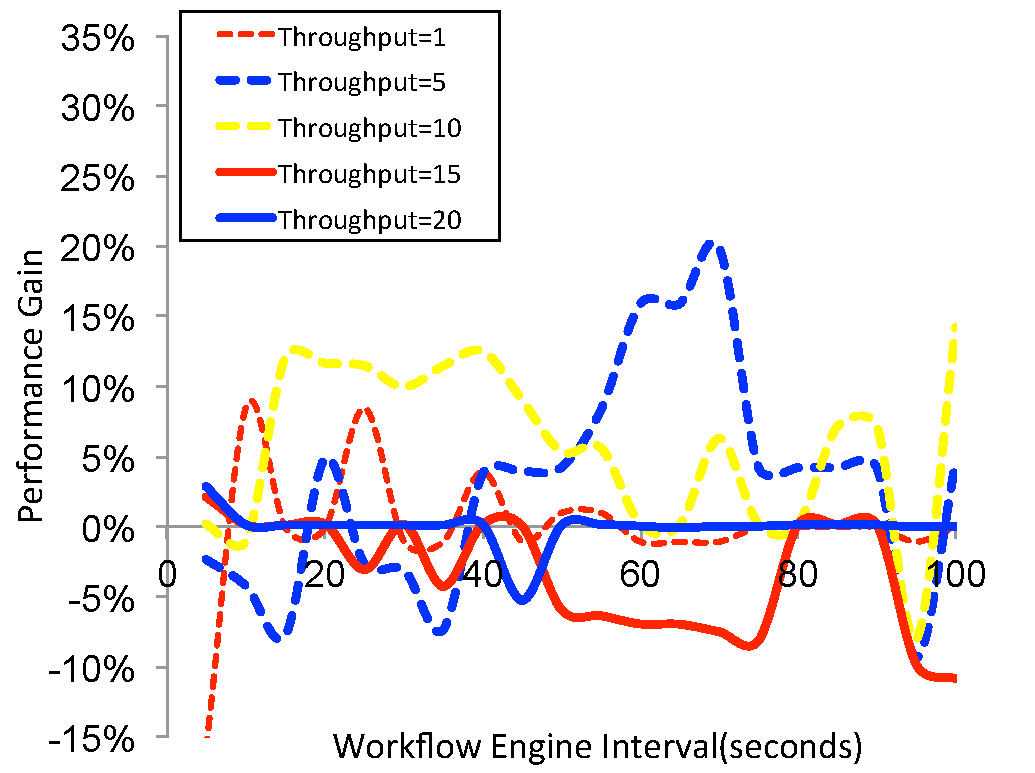
\includegraphics[width=0.9\linewidth]{figure/MAX-MIN-Broadband.pdf}
  \captionof{figure}{Broadband }
  \label{fig:MAX-MIN-Broadband}
  \vspace{-10pt}
\end{figure}

\begin{figure}[!htb]
\centering
 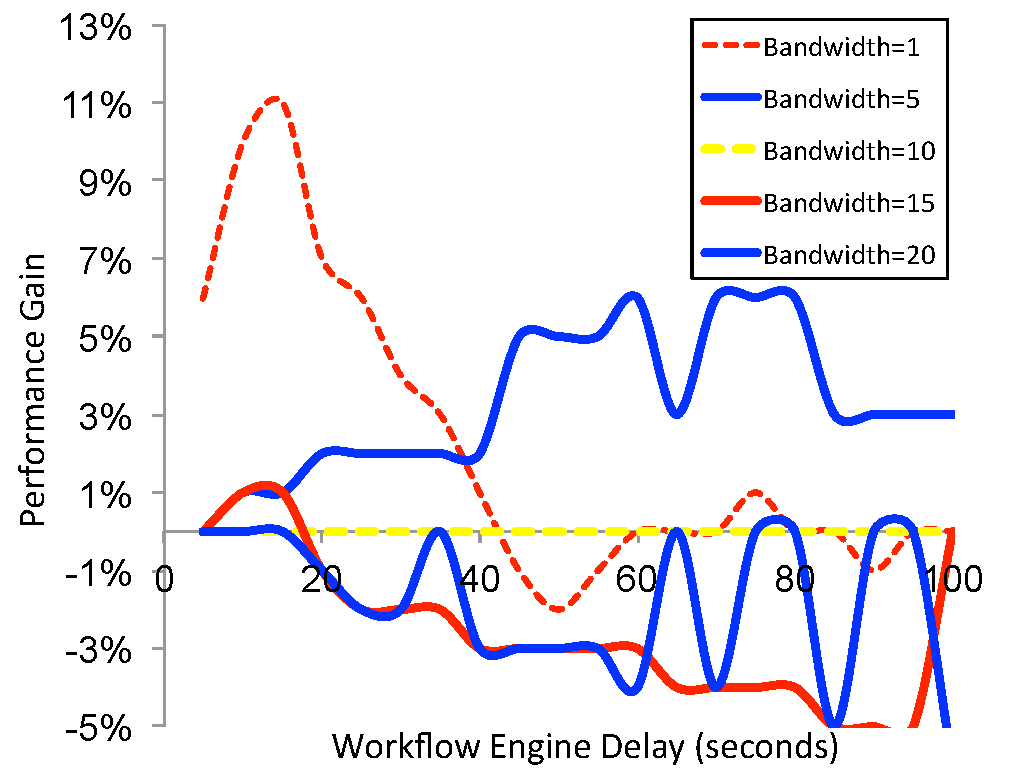
\includegraphics[width=0.9\linewidth]{figure/MAX-MIN-CyberShake.pdf}
  \captionof{figure}{CyberShake}
  \label{fig:MAX-MIN-CyberShake}
  \vspace{-10pt}
\end{figure}

\begin{figure}[!htb]
\centering
 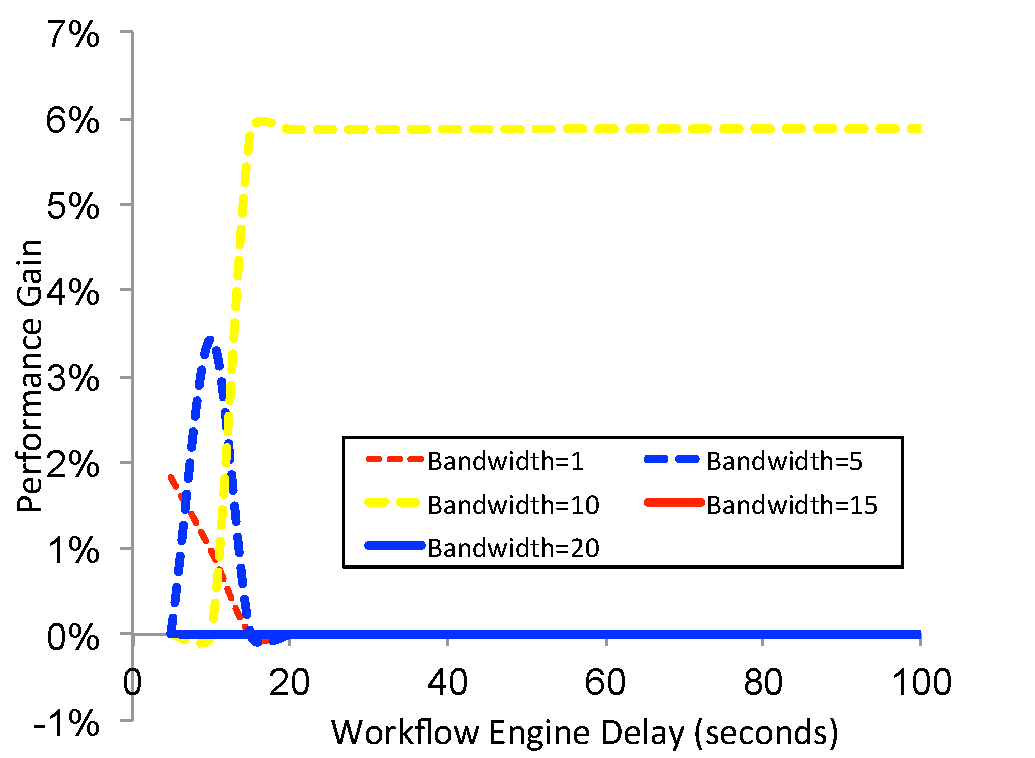
\includegraphics[width=0.9\linewidth]{figure/MAX-MIN-Montage.pdf}
  \captionof{figure}{Montage}
  \label{fig:MAX-MIN-Montage}
  \vspace{-10pt}
\end{figure}


Experiment 1: Fig.~\ref{fig:MAX-MIN-Broadband},~\ref{fig:MAX-MIN-CyberShake},~\ref{fig:MAX-MIN-Montage} show the  \emph{Performance Gain} of MAXMIN over MINMIN for the three workflows. We expected to see most  \emph{Performance Gain} $>0$ if MAXMIN is a overhead robust heuristic compared to MINMIN. However, except for the Montage workflow, the \emph{Performance Gain} is not significant for all of parameter settings, which concludes that MAXMIN is not globally overwhelming MINMIN in terms of overhead robustness. The reason we believe is that the  \emph{Performance Gain} in this comparison highly depends on the ratio of job runtime, workflow engine delay, number of resources and throughput of workflow engine. 

\begin{figure}[!htb]
\centering
 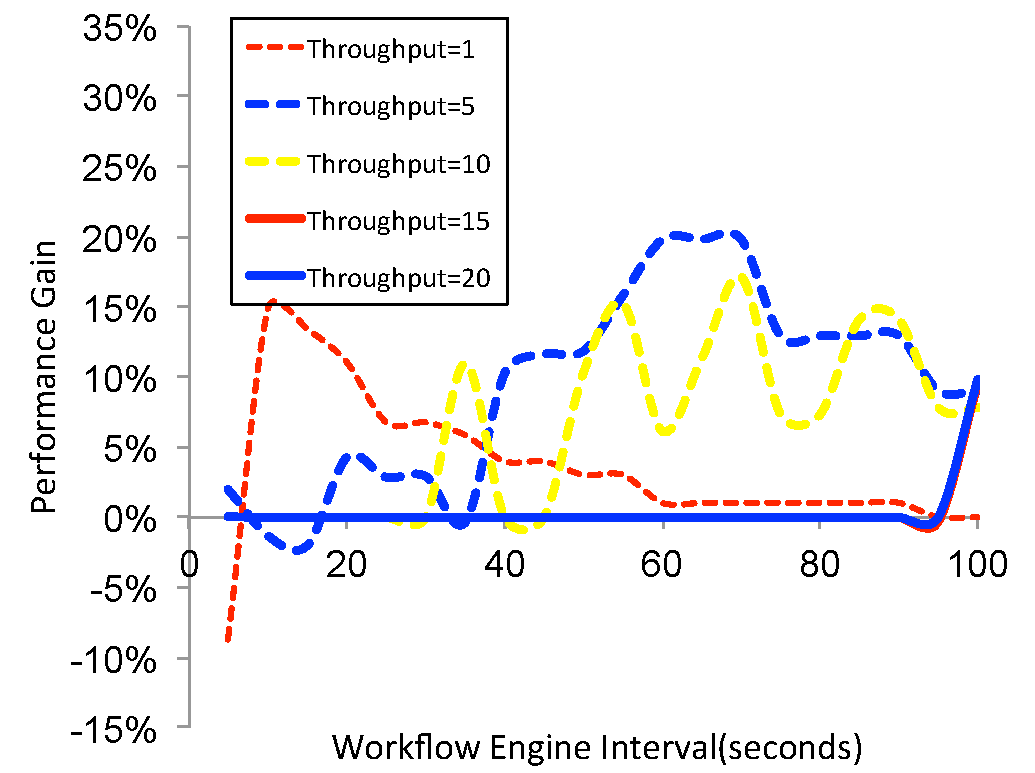
\includegraphics[width=0.9\linewidth]{figure/DFS-BFS-Broadband.pdf}
  \captionof{figure}{Broadband }
  \label{fig:DFS-BFS-Broadband}
  \vspace{-10pt}
\end{figure}

\begin{figure}[!htb]
\centering
 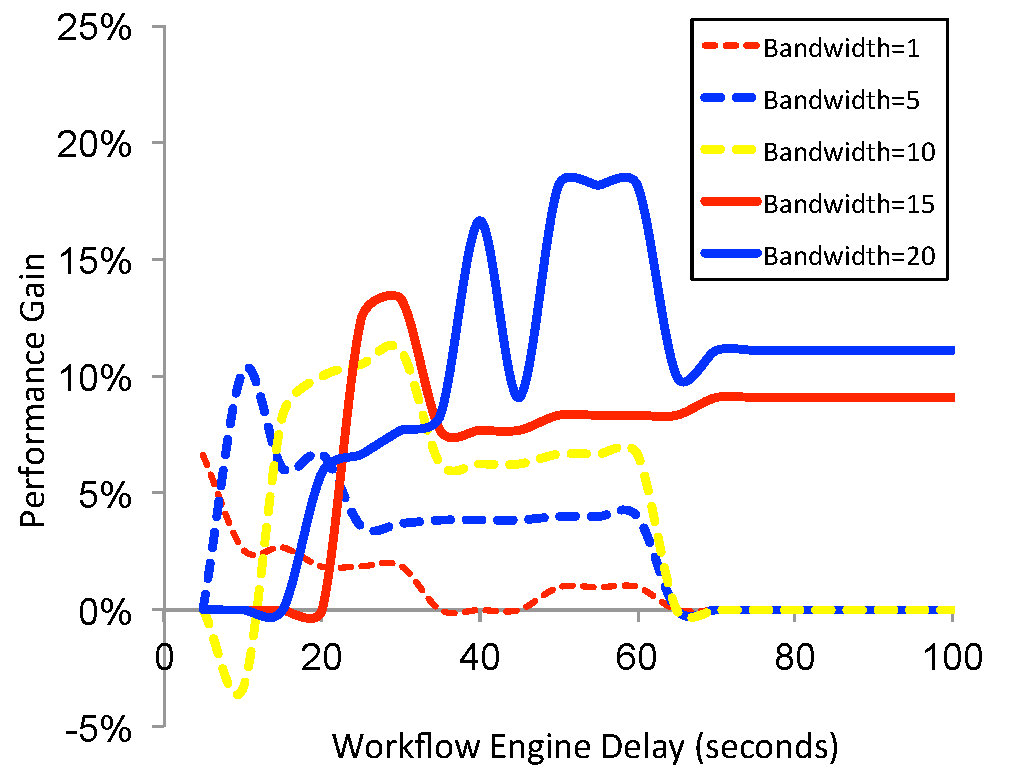
\includegraphics[width=0.9\linewidth]{figure/DFS-BFS-CyberShake.pdf}
  \captionof{figure}{CyberShake}
  \label{fig:DFS-BFS-CyberShake}
  \vspace{-10pt}
\end{figure}

\begin{figure}[!htb]
\centering
 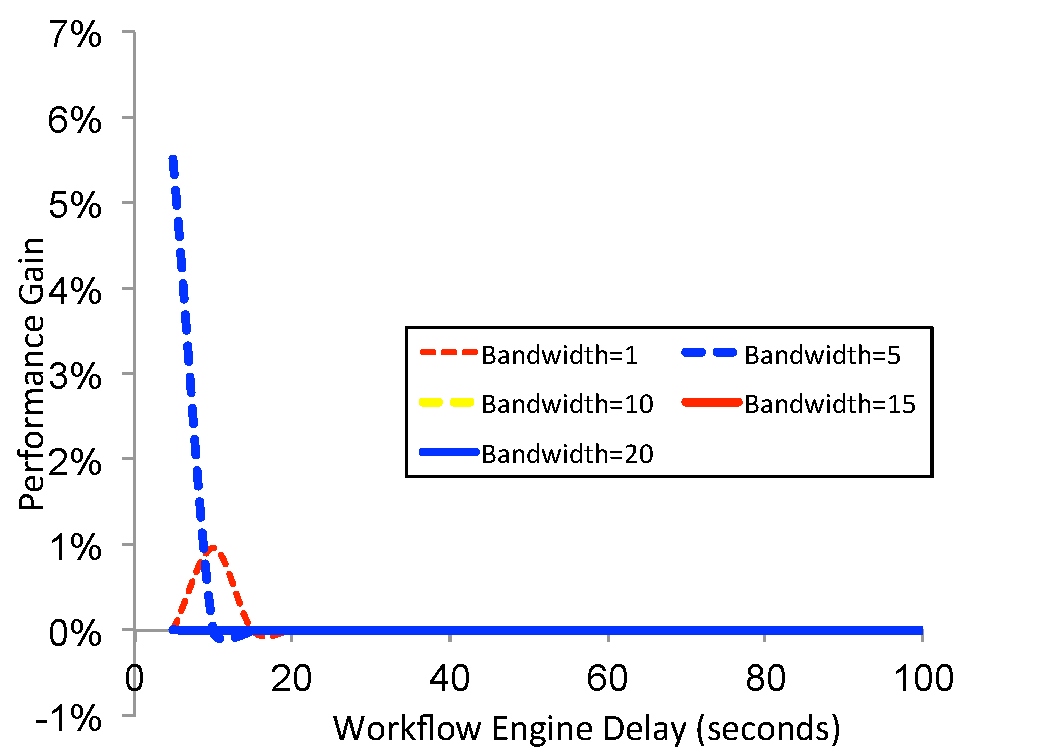
\includegraphics[width=0.9\linewidth]{figure/DFS-BFS-Montage.pdf}
  \captionof{figure}{Montage}
  \label{fig:DFS-BFS-Montage}
  \vspace{-10pt}
\end{figure}


Experiment 2: Fig.~\ref{fig:DFS-BFS-Broadband},~\ref{fig:DFS-BFS-CyberShake},~\ref{fig:DFS-BFS-Montage} show the \emph{Performance Gain} of BFS over DFS for the three workflows. We observe that most  \emph{Performance Gain} $>0$ and thus BFS performs better than DFS in terms of overhead robustness. What is more, Fig~\ref{fig:DFS-BFS-CyberShake} shows with the increase of average throughput, the \emph{Performance Gain} is more significant. We can also see that when the average throughput is high, the \emph{Performance Gain} increases with the average interval of workflow engine. This suggests us in a real environment with a large overhead, we should use BFS instead of DFS. 


\begin{figure}[!htb]
\centering
 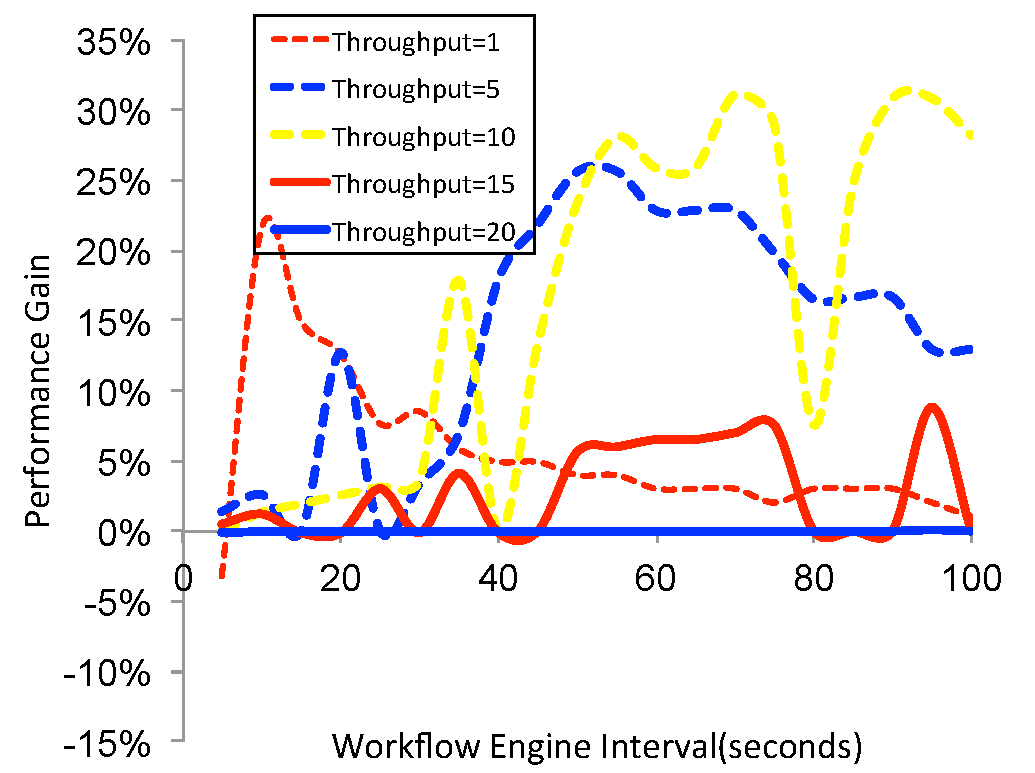
\includegraphics[width=0.9\linewidth]{figure/UFFS-FFS-Broadband.pdf}
  \captionof{figure}{Broadband }
  \label{fig:UFFS-FFS-Broadband}
  \vspace{-10pt}
\end{figure}

\begin{figure}[!htb]
\centering
 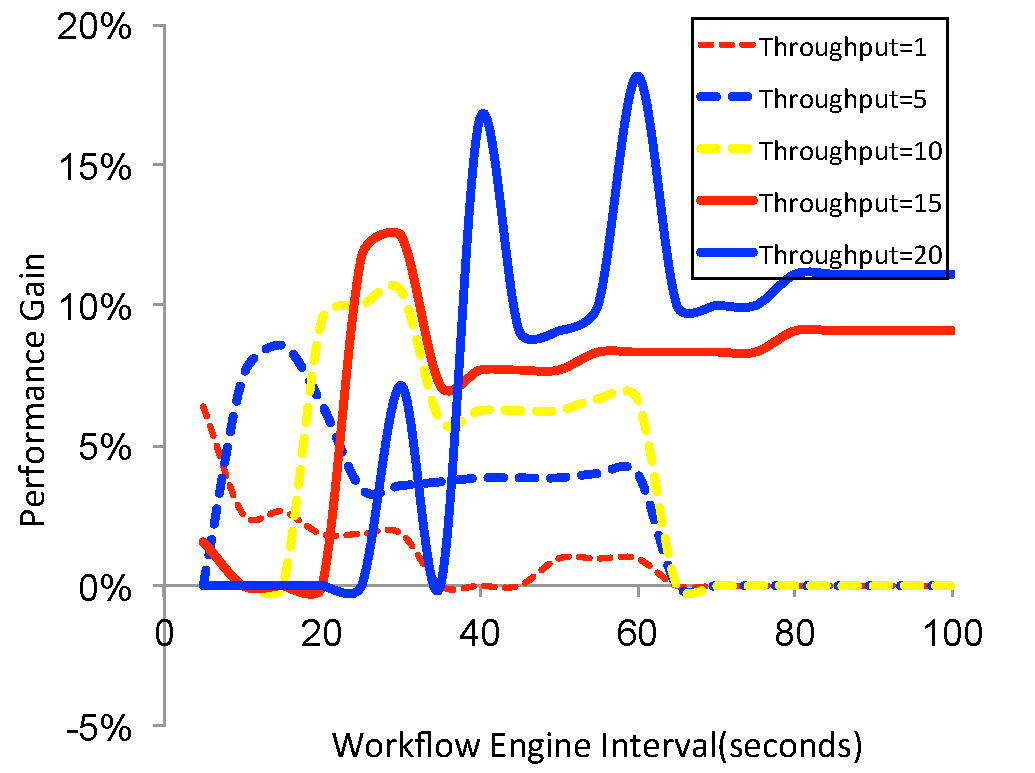
\includegraphics[width=0.9\linewidth]{figure/UFFS-FFS-CyberShake.pdf}
  \captionof{figure}{CyberShake}
  \label{fig:UFFS-FFS-CyberShake}
  \vspace{-10pt}
\end{figure}

\begin{figure}[!htb]
\centering
 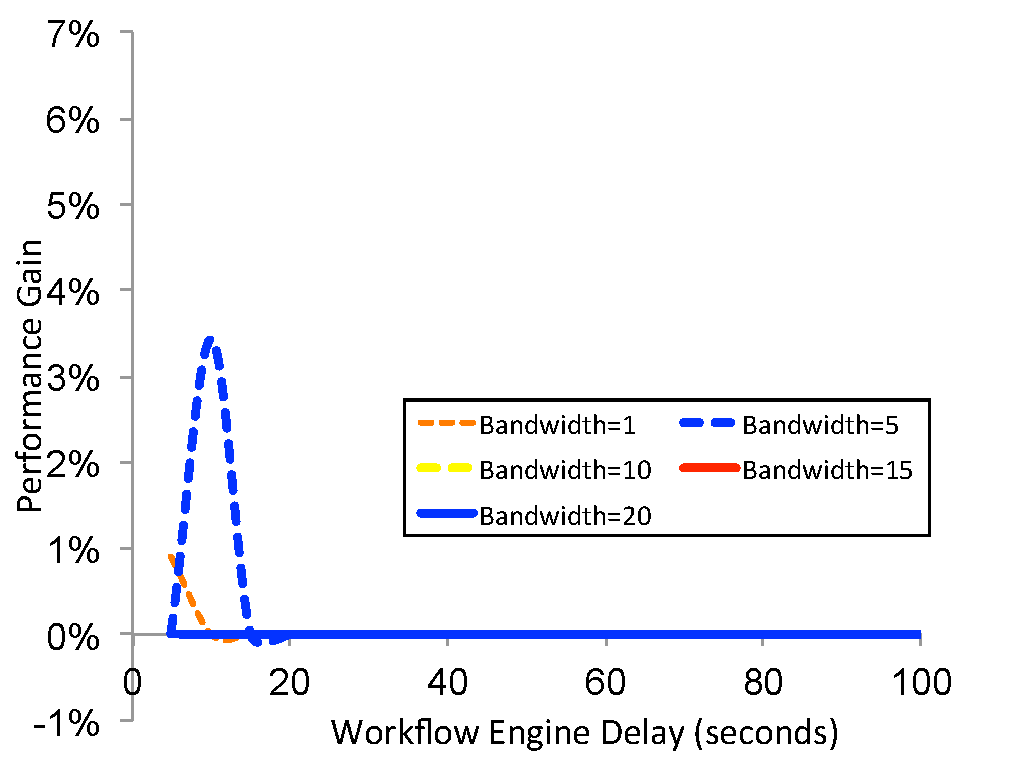
\includegraphics[width=0.9\linewidth]{figure/UFFS-FFS-Montage.pdf}
  \captionof{figure}{Montage}
  \label{fig:UFFS-FFS-Montage}
  \vspace{-10pt}
\end{figure}



Experiment 3: Fig.~\ref{fig:UFFS-FFS-Broadband},~\ref{fig:UFFS-FFS-CyberShake},~\ref{fig:UFFS-FFS-Montage} show the \emph{Performance Gain} of FFS over UFFS for the three workflows. We observe that most  \emph{Performance Gain} $>0$ and thus FFS performs better than UFFS in terms of overhead robustness, which is similar to Experiment 2. Comparing Fig.~\ref{fig:DFS-BFS-Broadband} and Fig.~\ref{fig:UFFS-FFS-Broadband} we can see the \emph{Performance Gain} of FFS over UFFS is more significant (30\%) than that of BFS over DFS (20\%).  
\begin{figure}[!htb]
\centering
 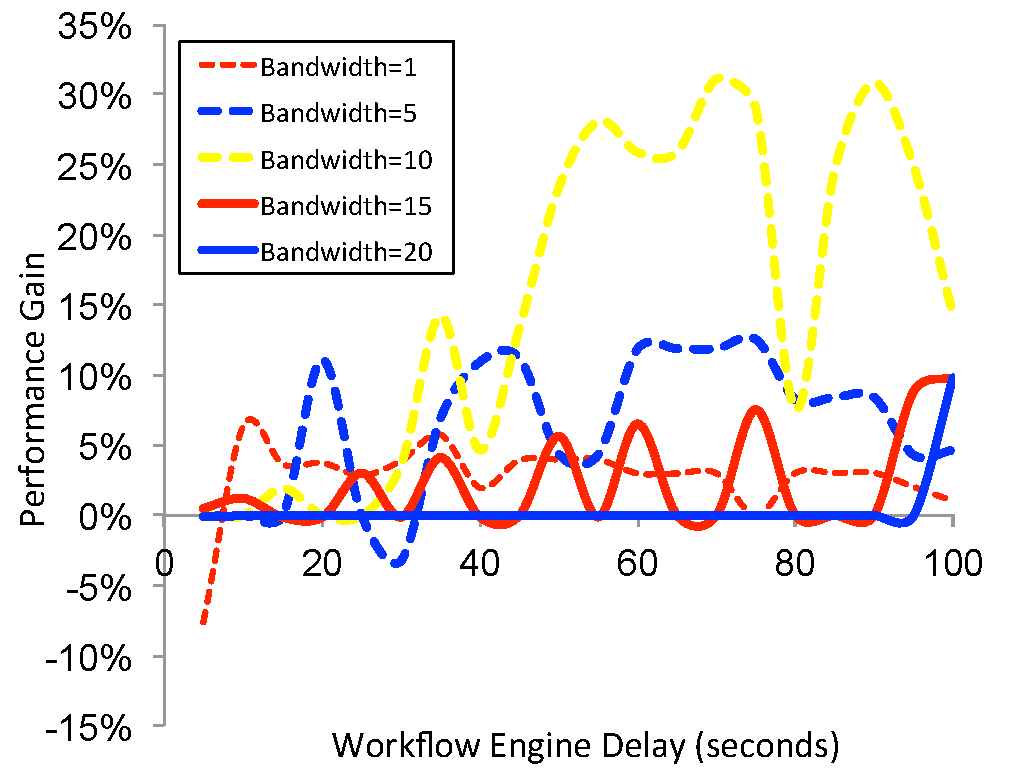
\includegraphics[width=0.9\linewidth]{figure/UIFS-IFS-Broadband.pdf}
  \captionof{figure}{Broadband }
  \label{fig:UIFS-IFS-Broadband}
  \vspace{-10pt}
\end{figure}

\begin{figure}[!htb]
\centering
 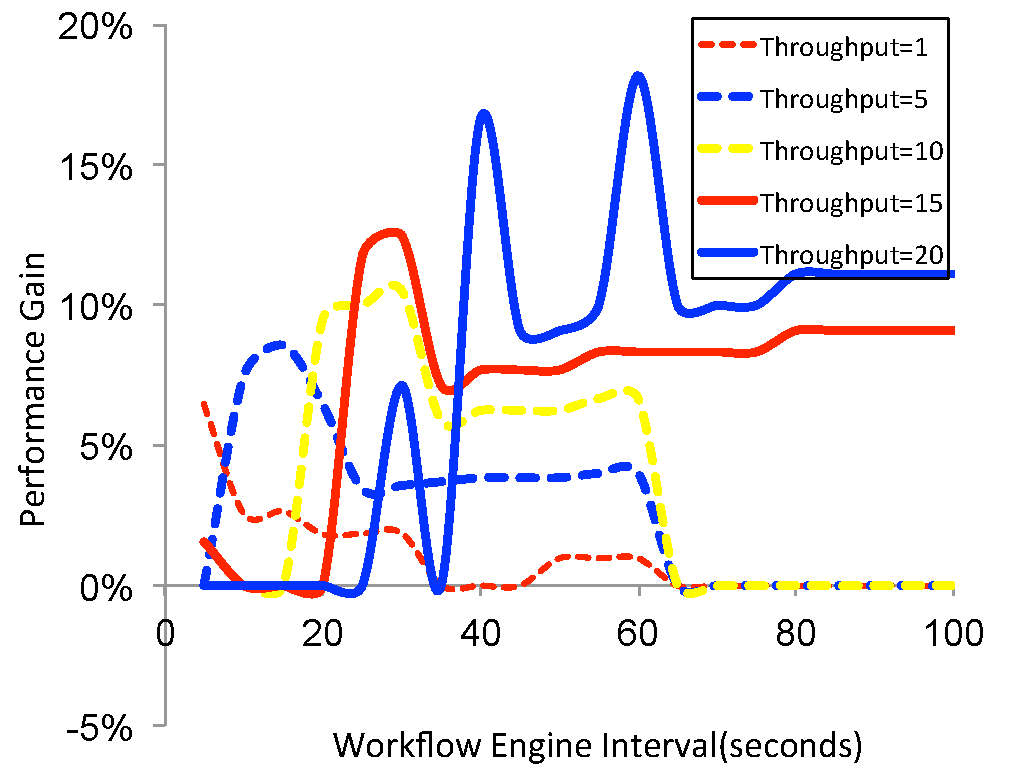
\includegraphics[width=0.9\linewidth]{figure/UIFS-IFS-CyberShake.pdf}
  \captionof{figure}{CyberShake}
  \label{fig:UIFS-IFS-CyberShake}
  \vspace{-10pt}
\end{figure}

\begin{figure}[!htb]
\centering
 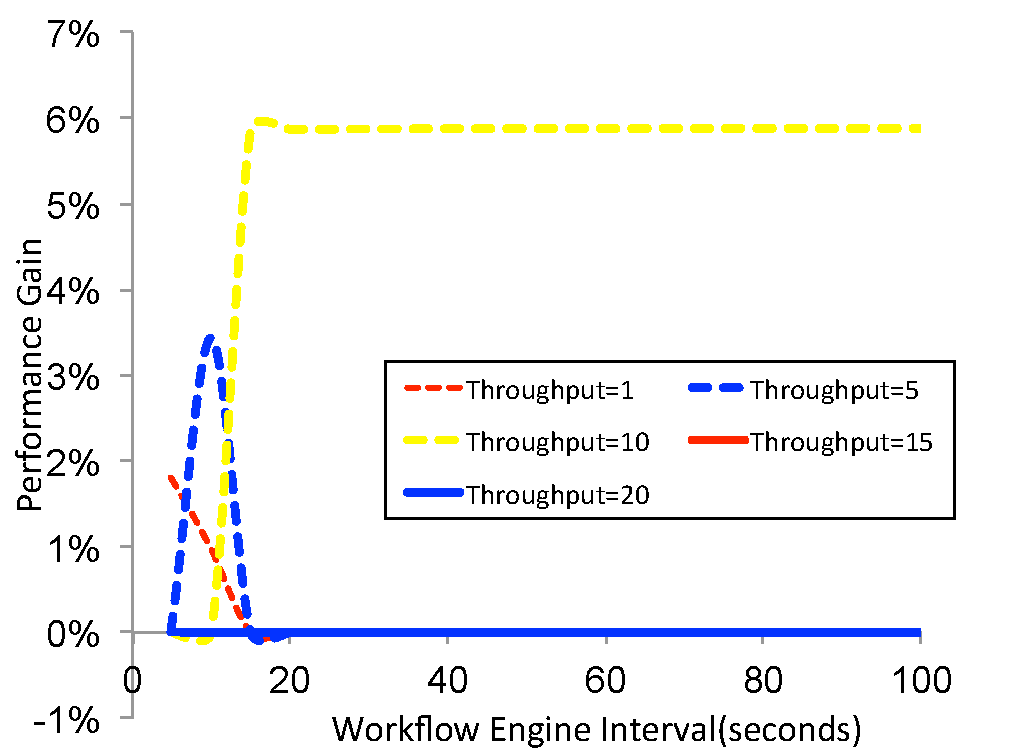
\includegraphics[width=0.9\linewidth]{figure/UIFS-IFS-Montage.pdf}
  \captionof{figure}{Montage}
  \label{fig:UIFS-IFS-Montage}
  \vspace{-10pt}
\end{figure}
Experiment 4: Fig.~\ref{fig:UIFS-IFS-Broadband},~\ref{fig:UIFS-IFS-CyberShake},~\ref{fig:UIFS-IFS-Montage} show the \emph{Performance Gain} of IFS over UIFS for the three workflows. We observe that most  \emph{Performance Gain} $>0$ and thus IFS performs better than UIFS in terms of overhead robustness, which is similar to Experiment 3. The reason is that for these workflows, IF based heuristics can produce similar schedule as the heuristics based on the number of children. Most of the workflows used in this paper is not irregular enough and thus we are not able to show the difference of IF based heuristics and the heuristics based on the number of children. 

\section{Conclusion and Future Work}





\bibliographystyle{IEEEtran}
\bibliography{IEEEabrv,biblio}


\end{document}

